\documentclass[border=4pt]{standalone}
\usepackage[T1]{fontenc}
\usepackage{tikz}
\usetikzlibrary{arrows.meta,positioning,fit,backgrounds,shapes.geometric,calc}
\definecolor{orch}{HTML}{234767}
\definecolor{ctx}{HTML}{EAF1F8}
\definecolor{retr}{HTML}{E2F0ED}
\definecolor{ext}{HTML}{F7EBDD}
\definecolor{infra}{HTML}{F1F3F5}
\tikzset{
 every node/.style={font=\sffamily\fontsize{8.5}{10}\selectfont,align=center,execute at begin node={\hyphenpenalty=10000\exhyphenpenalty=10000}},
 block/.style={draw=orch!80,fill=white,rounded corners=1.5pt,minimum height=7mm,inner sep=3pt,line width=.55pt},
 context/.style={block,fill=ctx},
 engine/.style={block,fill=orch,text=white},
 retrieval/.style={block,fill=retr},
 external/.style={block,fill=ext},
 storage/.style={block,fill=infra},
 optional/.style={dashed},
 flow/.style={-{Stealth[length=2mm]},draw=orch!90,line width=.65pt},
 control/.style={flow,dashed},
 error/.style={flow,densely dotted},
 group/.style={draw=orch!50,rounded corners=3pt,inner sep=5pt,line width=.5pt},
 heading/.style={font=\sffamily\bfseries\fontsize{8.5}{10}\selectfont,text=orch},
 edgelabel/.style={font=\sffamily\fontsize{7.5}{9}\selectfont,fill=white,inner sep=1pt,text=orch}
}

\begin{document}
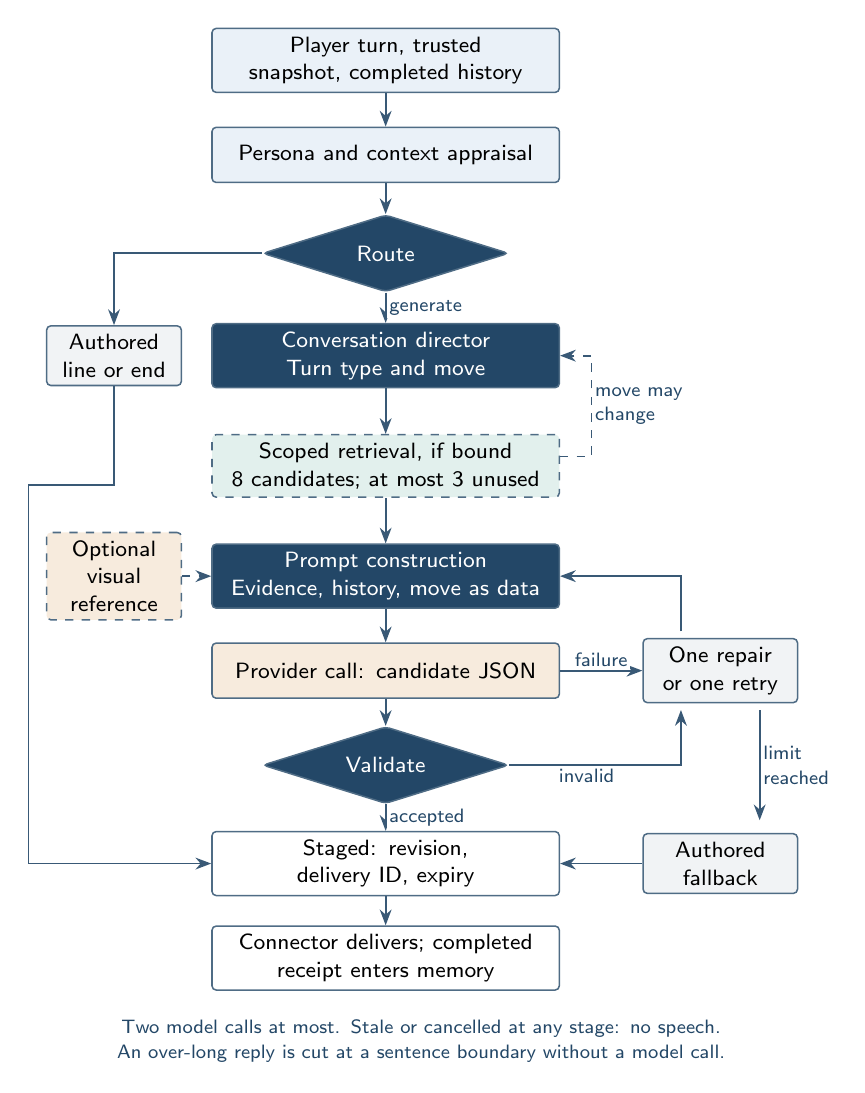
\begin{tikzpicture}
\node[context,text width=4.2cm] (input) at (0,12.4) {Player turn, trusted snapshot, completed history};
\node[context,text width=4.2cm] (context) at (0,11.2) {Persona and context appraisal};
\node[engine,diamond,aspect=3.2,text width=2.5cm,inner sep=0pt] (route) at (0,9.95) {Route};
\node[engine,text width=4.2cm] (director) at (0,8.65) {Conversation director\\Turn type and move};
\node[retrieval,optional,text width=4.2cm] (retrieve) at (0,7.25) {Scoped retrieval, if bound\\8 candidates; at most 3 unused};
\node[engine,text width=4.2cm] (pack) at (0,5.85) {Prompt construction\\Evidence, history, move as data};
\node[external,text width=4.2cm] (candidate) at (0,4.65) {Provider call: candidate JSON};
\node[engine,diamond,aspect=3.2,text width=2.5cm,inner sep=0pt] (check) at (0,3.45) {Validate};
\node[block,text width=4.2cm] (stage) at (0,2.2) {Staged: revision, delivery ID, expiry};
\node[block,text width=4.2cm] (receipt) at (0,1) {Connector delivers; completed receipt enters memory};
\node[storage,text width=1.5cm] (authored) at (-3.45,8.65) {Authored line or end};
\node[external,optional,text width=1.5cm] (vision) at (-3.45,5.85) {Optional visual reference};
\node[storage,text width=1.75cm] (repair) at (4.25,4.65) {One repair or one retry};
\node[storage,text width=1.75cm] (fallback) at (4.25,2.2) {Authored fallback};
\draw[flow] (input) -- (context);
\draw[flow] (context) -- (route);
\draw[flow] (route) -- node[edgelabel,right]{generate} (director);
\draw[flow] (director) -- (retrieve);
\draw[flow] (retrieve) -- (pack);
\draw[flow] (pack) -- (candidate);
\draw[flow] (candidate) -- (check);
\draw[flow] (check) -- node[edgelabel,right]{accepted} (stage);
\draw[flow] (stage) -- (receipt);
\draw[flow] (route.west) -| (authored.north);
\draw[flow] (authored.south) -- ($(authored.south)+(0,-1.25)$) -| ($(vision.west)+(-.22,0)$) |- ($(stage.west)$);
\draw[control] (vision) -- (pack);
\draw[control] ($(retrieve.east)+(0,.12)$) -- ++(.4,0) |- node[edgelabel,pos=.25,right,text width=1.7cm,align=left]{move may change} (director.east);
\draw[flow] (candidate) -- node[edgelabel,above]{failure} (repair);
\draw[flow] (check.east) -- node[edgelabel,below,pos=.45]{invalid} (3.75,3.45) -- (3.75,4.15);
\draw[flow] (3.75,5.15) |- (pack.east);
\draw[flow] (4.75,4.15) -- node[edgelabel,right,text width=.9cm,align=left]{limit reached} (4.75,2.75);
\draw[flow] (fallback) -- (stage);
\node[edgelabel,text width=8.6cm] at (.45,-.05) {Two model calls at most. Stale or cancelled at any stage: no speech. An over-long reply is cut at a sentence boundary without a model call.};
\end{tikzpicture}
\end{document}
